\documentclass[a4paper, 12pt]{article}
\usepackage{graphicx,hyperref,float,comment,listings,amsmath,longtable,geometry,caption,ragged2e,svg}
\lstdefinestyle{mystyle}{
	basicstyle=\small,
	breaklines=true,
	numbers=left,
	numberstyle=\tiny,
	numbersep=5pt,
}
\lstset{style=mystyle}
\graphicspath{{images/}}
\hypersetup{
	colorlinks=true,
	linkcolor=blue,
	filecolor=magenta,      
	urlcolor=cyan,
}

\title{\Large\textbf{Suppression d'imprimante et traitement des données sur le Lambda 9}}
\author{Gaëtan PINOT}
\date{Avril 2024}

\begin{document}
\pagenumbering{gobble}
%Page de titre
\maketitle

\newpage

\pagenumbering{arabic}

\section{Câblage}\label{cablage}


La station de traitement de données du Lambda 9 est normalement connectée à une imprimante par un port DB25, le standard de communication entre les deux est RS232.
Le standard RS232 permet d'utiliser un port série standard DE9\footnote{DE9 est le nom correct du port plus souvent appelé DB9 %\url{https://fr.wikipedia.org/wiki/D-sub}
}.
Pour pouvoir remplacer l'imprimante par un ordinateur il faut un cable de conversion entre le port DB25 et le port DB9 de l'ordinateur.


\begin{table}[htb]
	\begin{tabular}{|c|c|}
		\hline
		Signal & N° de pin DB25 \\ \hline
		TD     & 2              \\ \hline
		RD     & 3              \\ \hline
		RTS    & 4              \\ \hline
		CTS    & 5              \\ \hline
		DSR    & 6              \\ \hline
		GND    & 1,7            \\ \hline
		CD     & 8              \\ \hline
		RESET  & 15             \\ \hline
		DTR    & 20             \\ \hline
	\end{tabular}
	\centering
	\caption{Schéma de câblage de la sortie imprimante du Lambda 9, directement tiré des dessins techniques}
	\label{table:pinoutLambda}
\end{table}

Les deux appareils sont des DTE\footnote{Data Terminal Equipement}, les convertisseurs classiques ne fonctionnent pas car certains fils doivent être croisés et certains signaux ne peuvent être généré par aucun des deux appareils.
Il faut un cable null-modem\footnote{Cable qui croisent certains fils permettant la communication entre DTE} standard DE9-DB25.
Ou le faire soit meme selon le schéma de la Figure \ref{fig:cableLambda}.


%%%
\begin{comment}
		\begin{table}[htb]
		\centering
		\begin{tabular}{|c|c|c|c|}
			\hline
			Signaux &DB9   & DB25    & Signaux\\ \hline\hline
			RD&2     & 2       &TD\\ \hline
			TD&3     & 3       &RD\\ \hline
			GND&5     & 7       &GND\\ \hline
			DSR&6     & 20      &DTR\\ \hline
			CD,DTR,CTS&1,4,8 & 4,5,6,8 &RTS,CTS,DSR,CD\\ \hline
		\end{tabular}
	\end{table}
	Ceci (figure \ref{fig:cableLambda}) est le schéma du seul câblage que j'ai réussi à faire fonctionner.
	Les signaux \verb|TD| et \verb|RD| sont croisés pour que les deux appareils puissent communiquer.
	Les signaux \verb|CD| sur les deux appareils sont reliés à d'autre signaux car il devrait normalement être généré par le DCE (i.e.\ l'imprimante).
	Les autos signaux (\verb|RTS|, \verb|CTS|, \verb|DSR|, \verb|DTR|) sont reliés entre eux pour que les deux appareils soit prêt dès le branchement du cable, pour simplifier le programme de réception des données. 
\end{comment}
%%%

\newpage
\section{Simuler l'imprimante pour recevoir des données}\label{simuler}


On commence par connecter l'ordinateur au Lambda 9 avec le cable null-modem.
Puis on met en place une connexion série entre l'ordinateur et le Lambda 9, ayant pour paramètres :
\begin{description}
	\item[Bauds] 9600 
	\item[Bits de données] 8 
	\item[Bit de stop] 1 
	\item[Parité] Aucune
	\item[Contrôle de flux] Matériel (RTS/CTS)
\end{description}


Une fois l'ordinateur connecté au Lambda 9, il faut simuler l'imprimante pour que le Lambda 9 puisse envoyer les données.
Le Lambda 9 va envoyer des chaines de caractère ASCII se terminant par un retour chariot\footnote{Différentes représentations du retour chariot: \texttt{<CR>},  \texttt{\textbackslash r}, \^{}M, dec:13, hex:0D}.
Il faut répondre par la chaine \verb|01\r| pour que le Lambda 9 continue d'envoyer les données.

\newpage
\section{Analyse des données}\label{analyse}

\subsection{En-tête}\label{en-tete}

Quand on lance une mesure de scan, le Lambda 9 commence par envoyer un en-tête qui contient les informations sur la mesure.\\
Les valeurs de paramètres du menu de scan du Lambda 9 sont notés \verb|VALEUR PARAM LMBD|, les valeurs notés \emph{Valeur} sont des valeurs données dans l'en-tête ou calculées.
Leur nom est explicite.\\
Voici un exemple d'en-tête :
\begin{lstlisting}
Z0
IT,Z0,F15936,416,0,200,D0128,1280,A1,X2100,-100,5,S2090.0,D1,1,Y110.0,-22.000,4,Z0,D0128,1280,L1
\end{lstlisting}
Les valeurs sont séparés par des virgules et on la signification suivante\footnote{Les valeurs qui ne sont pas expliquées sont des valeurs qui ne change pas peu importe les paramètres de mesure}:
\begin{description}
	\item[Z0]
	\item[IT]
	\item[Z0]
	\item[F15936] \emph{ValEchelleMax}, la valeur réel qui correspond à l'échelle maximal des données envoyées, ici 15936.
	\item[416] \emph{ValEchelleMin}, la valeur réel qui correspond à l'échelle minimal des données envoyées, ici 416.
	\item[0]
	\item[200]
	\item[D0128]  \emph{FacteurVitesse}, facteur de vitesse de balayage , ici 128.
		Change quand la vitesse de balayage (\verb|SCAN SPEED|) ou le format de l'abscisse (\verb|ABSCISSA FORMAT|) change.
		\textbf{IMPORTANT}, pour certaines valeurs de \verb|ABSCISSA FORMAT|, le facteur de vitesse ne change pas avec \verb|SCAN SPEED|, exemples en Table \ref{tab:ValeursFacteurVitesse}.
		Il est impossible de déduire avec certitude la vitesse de balayage pour certaines valeurs de \verb|ABSCISSA FORMAT|.
	\item[1280] \emph{InconnuAbscisse}, valeur inconnue qui change quand \verb|ABSCISSA FORMAT| change, voir Table \ref{tab:ValeursFacteurVitesse}, ici 1280. 
	\item[A1]
	\item[X2100] \emph{InconnuLongueurOnde}, valeur inconnu qui correspond à \emph{LongueurOndeMax} arrondie au multiple de 100 supérieur, ici 2100.
	\item[-100] \emph{FacteurFormatAbscisse}, permet de calculer la valeur \verb|ABSCISSA FORMAT|, ici -100.
	\item[5] \emph{DiviseurFormatAbscisse}, permet de calculer la valeur \verb|ABSCISSA FORMAT|, ici 5.
	\item[S2090.0] \emph{LongueurOndeMax}, valeur de longueur d'onde maximal mesurée en nm, ici 2090.0.
	\item[D1]
	\item[1]
	\item[Y110.0] \emph{EchelleMax}, valeur maximal enregistré par le Lambda 9, ici 110.0.
		Correspond à la valeur \verb|ORD MAX| sur le Lambda 9.
	\item[-22.000] \emph{Décalage}, sert à calculer l'échelle minimal, ici $-22.000$.
	\item[4]
	\item[Z0]
	\item[D0128] Duplicata de \emph{FacteurVitesse}.
	\item[1280] Duplicata de \emph{InconnuAbscisse}.
	\item[L1] \emph{StyleDeLigne}, style de la ligne de courbe de mesure à l'impression, peut être \{1,2,3,4\}, ici 1.
		Correspond à la valeur \verb|DASH| sur le Lambda 9.\\

\end{description}


Valeurs que l'on calcule à partir des valeurs de l'en-tête:

\begin{description}
	\item[EchelleMin] Valeur minimal enregistré par le Lambda 9, ici 0.
		Calculé avec la formule : 
		$$ \text{EchelleMax} + ( \text{Décalage} \times 5 ) = \text{EchelleMin}$$
		Ici :
		$$110.0 + ( -22.000 \times 5 ) = 0.0$$ 
		Correspond à la valeur \verb|ORD MIN| sur le Lambda 9.

	\item[FormatAbscisse] Format de l'abscisse de l'imprimante en nm/cm. 
		Calculé avec la formule : 
		$$ { - \frac{FacteurFormatAbscisse}{DiviseurFormatAbscisse} } = FormatAbscisse $$ 
		Ici :
		$$ - \frac{-100}{5} = 20$$ 
		Correspond à la valeur \verb|ABSCISSA FORMAT| sur le Lambda 9.

	\item[VitesseDeBalayage] Vitesse de balayage en nm/min, ici 240. 
		\textbf{IMPORTANT}, le calcule change en fonction de \emph{FormatAbscisse}, voir Table \ref{tab:ValeursFacteurVitesse}.
		Calculé avec la formule : 
		$$FacteurVitesse \times 0,9375 \times 2 = VitesseDeBalayage$$
		Pour $ FormatAbscisse = 20 $.
		\\
		Ici :
		$$128 \times 0,9375 \times 2 = 240$$ 
		Correspond à la valeur \verb|SCAN SPEED| sur le Lambda 9.



\end{description}


\subsection{Valeurs mesurées}\label{valeurs}

Après l'en-tête viennent les valeurs mesurées sur 14 bits non signés $[0;16384]$. 
Exemple court\footnote{Il n'y a que 8 valeurs ici, mais il y en a 300 en réalité}:  

\begin{lstlisting}
14299
14330
14375
14338
14331
14351
14336
14331
\end{lstlisting}

On calcule les valeur suivantes: 

\begin{description}
	\item[LongueurOndeMini] On utilise le nombre de valeurs total, \emph{NombreValeurs}, pour determiner la valeur minimale de longueur d'onde de cette manière :
		\begin{multline*}
			 LongueurOndeMax - \left ( \frac{VitesseDeBalayage}{60} \times \frac{NombreValeurs}{20} \right ) 
			\\ = LongueurOndeMini 
\end{multline*}
		Le Lambda 9 envoie 20 valeurs par seconde de mesure.\\
		On divise le nombre de valeurs par 20 pour obtenir le nombre de secondes de mesure.\\
		On multiplie ce nombre par la vitesse de balayage, divisé par 60 pour avoir des nm/sec, pour obtenir la différence de longueur d'onde entre la première et la dernière valeur.
		Ici :
		$$ 2090 - \left ( \frac{240}{60} \times \frac{300}{20} \right ) = 2030 $$ \\


	\item[ValeurConvertie] On utilise cette formule pour convertir dans le format choisi pour l'ordonnée :
		\begin{multline*}
		 \left ( \frac{Valeur - ValEchelleMin}{ValEchelleMax} \times (EchelleMax - EchelleMin) \right ) 
			\\ + EchelleMin = ValeurConvertie 
			\end{multline*}
		Ici, 416 correspond à la valeur d'échelle minimal et 15936 à la valeur d'échelle maximal, si la valeurs sorte de cette plage, il y à une marge jusqu'à 0 et 16384.
		Par exemple, la valeur 14299 correspond à 95.8\%: 
		$$ \left (\frac{14299-416}{15936} \times ( 110 - 0 ) \right ) + 0 = 95.8$$\\

\end{description}

\newpage
\section{Annexe}\label{annexe}

		\begin{longtable}[c]{|c|c|c|c|}

\hline
\verb|SCAN SPEED| & \verb|ABSCISSA FORMAT| & \emph{FacteurVitesse} & \emph{InconnuAbscisse} \\ \hline
\endhead
%
0.9375     & 0.2             & 5              & 128     \\ \hline
1.875      & 0.2             & 10             & 128     \\ \hline
3.75       & 0.2             & 20             & 128     \\ \hline
7.5        & 0.2             & 40             & 128     \\ \hline
15         & 0.2             & 80             & 128     \\ \hline
30         & 0.2             & 160            & 128     \\ \hline
0.9375     & 1               & 5              & 640     \\ \hline
1.875      & 1               & 10             & 640     \\ \hline
3.75       & 1               & 20             & 640     \\ \hline
7.5        & 1               & 40             & 640     \\ \hline
15         & 1               & 80             & 640     \\ \hline
30         & 1               & 160            & 640     \\ \hline
60         & 1               & 320            & 640     \\ \hline
120        & 1               & 640            & 640     \\ \hline
0.9375     & 2               & 5              & 1280    \\ \hline
1.875      & 2               & 10             & 1280    \\ \hline
3.75       & 2               & 20             & 1280    \\ \hline
7.5        & 2               & 40             & 1280    \\ \hline
15         & 2               & 80             & 1280    \\ \hline
30         & 2               & 160            & 1280    \\ \hline
60         & 2               & 320            & 1280    \\ \hline
120        & 2               & 640            & 1280    \\ \hline
240        & 2               & 1280           & 1280    \\ \hline
0.9375     & 5               & 5              & 3200    \\ \hline
1.875      & 5               & 10             & 3200    \\ \hline
3.75       & 5               & 20             & 3200    \\ \hline
7.5        & 5               & 40             & 3200    \\ \hline
15         & 5               & 80             & 3200    \\ \hline
30         & 5               & 160            & 3200    \\ \hline
60         & 5               & 320            & 3200    \\ \hline
120        & 5               & 640            & 3200    \\ \hline
240        & 5               & 1280           & 3200    \\ \hline
480        & 5               & 2560           & 3200    \\ \hline
0.9375     & 10              & 1              & 1280    \\ \hline
1.875      & 10              & 2              & 1280    \\ \hline
3.75       & 10              & 4              & 1280    \\ \hline
7.5        & 10              & 8              & 1280    \\ \hline
15         & 10              & 16             & 1280    \\ \hline
30         & 10              & 32             & 1280    \\ \hline
60         & 10              & 64             & 1280    \\ \hline
120        & 10              & 128            & 1280    \\ \hline
240        & 10              & 256            & 1280    \\ \hline
480        & 10              & 512            & 1280    \\ \hline
960        & 10              & 1024           & 1280    \\ \hline
0.9375     & 20              & 1              & 1280    \\ \hline
1.875      & 20              & 1              & 1280    \\ \hline
3.75       & 20              & 2              & 1280    \\ \hline
7.5        & 20              & 4              & 1280    \\ \hline
15         & 20              & 8              & 1280    \\ \hline
30         & 20              & 16             & 1280    \\ \hline
60         & 20              & 32             & 1280    \\ \hline
120        & 20              & 64             & 1280    \\ \hline
240        & 20              & 128            & 1280    \\ \hline
480        & 20              & 256            & 1280    \\ \hline
960        & 20              & 512            & 1280    \\ \hline
0.9375     & 50              & 1              & 1600    \\ \hline
1.875      & 50              & 1              & 1600    \\ \hline
3.75       & 50              & 1              & 1600    \\ \hline
7.5        & 50              & 2              & 1600    \\ \hline
15         & 50              & 4              & 1600    \\ \hline
30         & 50              & 8              & 1600    \\ \hline
60         & 50              & 16             & 1600    \\ \hline
120        & 50              & 32             & 1600    \\ \hline
240        & 50              & 64             & 1600    \\ \hline
480        & 50              & 128            & 1600    \\ \hline
960        & 50              & 256            & 1600    \\ \hline
0.9        & 100             & 1              & 1600    \\ \hline
1.8        & 100             & 1              & 1600    \\ \hline
3.75       & 100             & 1              & 1600    \\ \hline
7.5        & 100             & 1              & 1600    \\ \hline
15         & 100             & 2              & 1600    \\ \hline
30         & 100             & 4              & 1600    \\ \hline
60         & 100             & 8              & 1600    \\ \hline
120        & 100             & 16             & 1600    \\ \hline
240        & 100             & 32             & 1600    \\ \hline
480        & 100             & 64             & 1600    \\ \hline
960        & 100             & 128            & 1600    \\ \hline

\caption{Valeurs de \emph{FacteurVitesse} et d'\emph{InconnuAbscisse} pour toutes les combinaisons possibles de vitesse de balayage et de format d'abscisse}

\label{tab:ValeursFacteurVitesse}\\
\end{longtable}

\begin{figure}[htb]
		\centering
		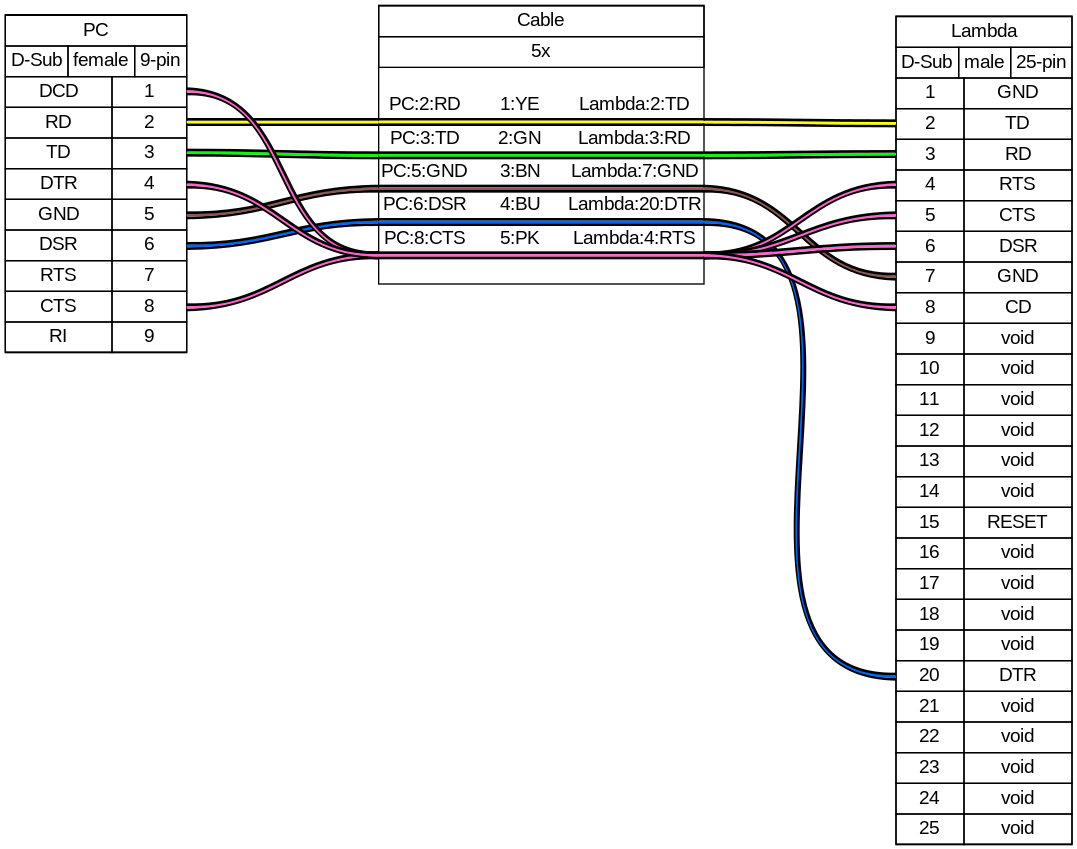
\includegraphics[width=1\textwidth]{cableLambda.png}
		\caption{Exemple de câblage fonctionnel entre l'ordinateur et le Lambda 9} % \protect \footnotemark}
		\label{fig:cableLambda}
	\end{figure}
	%\footnotetext{Schéma généré grâce à WireViz : \url{https://github.com/wireviz/WireViz}}



\end{document}
